\chapter{کاربردها}
ماتع و افزونه‌هایش در سال‌های اخیر کاربردهای گوناگونی پیدا کرده‌اند. در این بخش قصد داریم به تعدادی از کاربردهای آن بپردازیم.

\section{تخمین عمر مفید باقی‌مانده}
فالکن\LTRfootnote{Falcon} و همکاران\cite{falcon2020neural} در تحقیقی عمر مفید باقی‌مانده وسایل مکانیکی استفاده شده در حوزه درمان و بهداشت را بررسی کرده‌اند. تخمین عمر مفید یک وسیله مکانیکی یکی از مسائل مهم در حوزه مدیریت سلامت و پیشگیری است. توانایی تخمین قابل اطمینان بودن آن منجر به بهود در برنامه‌ریزی نگهداری و کاهش هزینه‌های مرتبط با آن می‌شود. در دسترس بودن سنسورهای با کیفیت بالا که چندین جنبه از اجزا را می‌سنجد این امکان را فراهم می‌کند که حجم زیادی از داده‌ها جمع‌آوری شود که این داده‌ها می‌تواند در تنظیم‌کردن مدل‌های برپایه داده\LTRfootnote{data-driven} استفاده شود.\cite{falcon2020neural}
\\

معماری مدل استفاده‌شده در تصویر ۴-۱ آورده شده است. داده‌ای که در حوزه بهداشت و پیشگیری استفاده می‌شود معمولا مقادیر اندازه‌گیری‌شده طولانی‌مدت سری‌های زمانی\LTRfootnote{Time Series} حس‌گرها هستند. 
سری زمانی‌های خام ورودی با پیش‌پردازش تبدیل به پنجره سری‌زمانی‌های کوچک‌تر می‌شوند. هر کدام از این پنجره‌ها به عنوان ورودی به یک شبکه از دو لایه پشته‌شده \lr{LSTM} به عنوان ورودی داده می‌شود و یک دنباله از ویژگی‌های استخراج‌شده حاصل می‌گردد. این ویژگی‌ها با ویژگی‌های خروجی یک ماتع الحاق می‌شود. نتیجه نهایی بعد از عبور از یک شبکه جلورو دو لایه پشته‌شده نهایی حاصل می‌گردد.\cite{falcon2020neural}
\\

\begin{figure}[!h]
\begin{center}
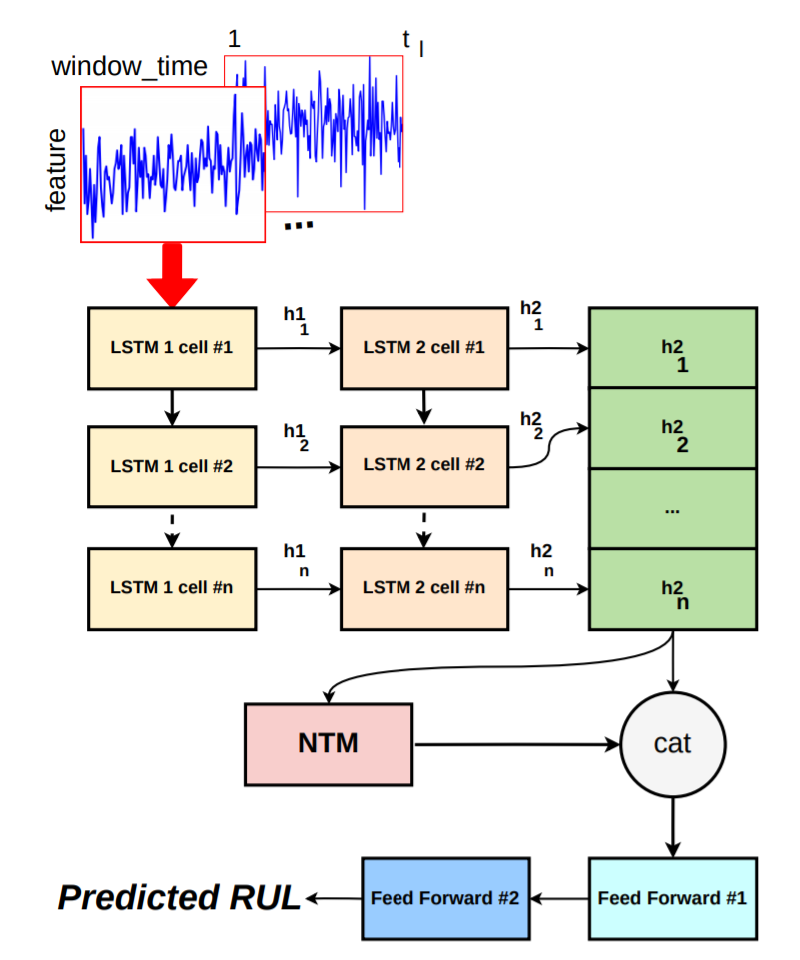
\includegraphics[height=14cm]{RUL.png}
\end{center}
\caption{معماری پیشنهادی برای کاربرد تخمین عمر مفید در کار تحقیقاتی فالکن و همکاران}
\medskip
\small
سری‌های زمانی ابتدا به پنجره‌های کوچک‌تر می‌شکنند سپس به عنوان ورودی به شبکه داده می‌شوند. ورودی از دو لایه \lr{LSTM} پشته‌شده می‌گذرد و سپس با خروجی یک ماتع الحاق می‌شود. در نهایت شبکه جلورو پشته‌شده مقدار تحمین عمر مفید را ارائه می‌دهند. 
\end{figure}

فالکن و همکاران معتقدند که وجود یک ماتع می‌تواند کمک به فهم بهتر الگوهای مخفی در داده‌ها و ذخیره‌سازی آن شود. در پژوهش آن‌ها کنترل‌گر ماتع را از نوع شبکه‌های جلورو برگزیدند.\cite{falcon2020neural} بهبود نتایج آن‌ها که در بخش پنجم به آن اشاره خواهد شد اثبات‌کننده نقش مثبت ماتع در مقاله آنان است.